\section{Introduction}

The dependency structure matrix genetic algorithm-II (DSMGA-II) is a model building GA proposed by Hsu and Yu in 2015~\cite{hsu:DSMGA2}.
Based on the dependency structure matrix (DSM), a new linkage model, called the incremental linkage set (ILS), is adopted in DSMGA-II to provide potential models for mixing. 
The restricted mixing and the back mixing are the major recombination operators of DSMGA-II. 
They are the keys to significantly reduce the number of function evaluations (NFE) compared with other optimal mixing operators. 
Experiment results show that DSMGA-II requires fewer function evaluations than the Linkage Tree Genepool Optimal Mixing Evolutionary Algorithm (LT-GOMEA)~\cite{bosman:LT-GOMEA} and Hierarchical Bayesian Optimization Algorithm (hBOA)~\cite{pelikan:hBOA}, two cutting-edge evolutionary algorithms, on various benchmark problems. 

However, there is still room for improvement with model building in DSMGA-II. 
In this paper, we propose a two-edge graphical linkage model, which is more expressive than the original DSM and customizes recombination for every single chromosome. 
We also demonstrate how the early-stop criterion reduces unnecessary trials and yields fewer function evaluations.

The remainder of this paper is organized as follows. 
Section 2 introduces the original DSMGA-II. 
Section 3 introduces the two-edge linkage model in detail, along with some new techniques to enhance mixing effectiveness. 
Section 4 shows the experiment results. 
Section 5 gives the summary and conclusion.



\section{DSMGA-II}
In this section, we first introduce the framework of DSMGA-II and the concept of incremental linkage set. 
Then we detail the restricted and back mixing operators, which are the kernel operators of DSMGA-II.

\begin{algorithm}
\caption{DSMGA-II}\label{algo_disjdecomp}
\SetKwData{Left}{left}\SetKwData{This}{this}\SetKwData{Up}{up}

\SetKwFunction{PopulationInitialization}{PopulationInitialization}
\SetKwFunction{GHC}{GHC}
\SetKwFunction{ShouldTerminate}{ShouldTerminate}
\SetKwFunction{TournamentSelection}{TournamentSelection}
\SetKwFunction{UpdateMatrix}{UpdateMatrix}
\SetKwFunction{RestrictedMixing}{RestrictedMixing}
\SetKwFunction{BackMixing}{BackMixing}

$P$: population, $S$: selected population, \\
$s$: selection pressure, $R$: constant, \\
$DSM$: dependency structure matrix, $M$: mask \\

\SetKwInOut{Input}{input}\SetKwInOut{Output}{output}
\Input{ $\ell$: problem size, $p$: population size }
\Output{ $P_{best}$ }

\BlankLine

$P \leftarrow$ \PopulationInitialization{$\ell$, $p$} \\
$P \leftarrow$ \GHC{$P$} \\
\While{not \ShouldTerminate}{
    $S \leftarrow$ \TournamentSelection{$P$, $s$} \\
    $DSM \leftarrow $ \UpdateMatrix{$S$} \\

    \For{$k\leftarrow 1$ \KwTo $R$}{
        $I \leftarrow$ random permutation from 1 to $p$ \\

        \For{$i \in I$}{
            $P_i$, $M \leftarrow$ \RestrictedMixing{$P_i$} \\
            \If{$M \neq \emptyset$} {
                $P \leftarrow$ \BackMixing{$P_i$, $M$} \\
            }
        }
    }
}
\Return best individual in $P$
\end{algorithm}


\subsection{Framework of DSMGA-II}
DSMGA-II consists of four major components: pair-wise linkage detection, model building, restricted mixing and back mixing. 
First, DSMGA-II randomly initializes a population. 
Then, in order to enhance the quality of pairwise linkage model and reduce the noise in the population, DSMGA-II performs a bit-flipping greedy hill climbing (GHC) on each chromosome. 
%For each randomly initialized chromosome, GHC randomly flips each bit in the chromosome and evaluates its fitness. 
%If the fitness improves, the chromosome accepts the change. Otherwise, the flipped bit is restored. 
Pairwise linkage detection was adopted in a later version of LTGA~\cite{pelikan:pairwise} and DSMGA~\cite{yu:DSMGA} due to its resistance to sampling noise. 
Performing GHC before linkage model building can further ensure the pairwise linkage information between genes, by ruling out trivial cases that can be solved without linkage information. 

After initializing the population, only the selected chromosomes are used to build the linkage model. 
The chromosomes are chosen by the tournament selection with selection pressure of 2, as suggested in~\cite{yu:population}. 
DSMGA-II adopts the mutual information as pairwise linkage measure and stores the linkage information in a DSM. 
Notice that the tournament selection is only performed to choose chromosomes for model building instead of updating the population. 
Then recombinations via the restricted and back mixings are proceeded with the original population. 
The pseudo code of DSMGA-II is given in Algorithm 1.

%Before mixing, DSMGA-II builds the ILS with the linkage information stored in DSM. The ILS is a set of models indicating possible subproblem structures. In the restricted mixing, the receiver tries to flip the bits within the model. If the fitness does not decrease, the receiver becomes a donor during the back mixing, and the new pattern is tried on all chromosomes in the population. The population is randomly shuffled in advance so that each chromosome takes turns acting as the receiver during the restricted mixing and the donor during the back mixing. The pseudo code of DSMGA-II is given in Algorithm 1. The detailed implementations of the ILS and the mixing operators are described in the following sections. 


\subsection{Incremental Linkage Set}
Before mixing, DSMGA-II builds the ILS with the linkage information stored in DSM. 
The DSM is an adjacent matrix representing the dependency between two variables, where each entry stores the pairwise information between two bits. 
In DSMGA-II, pairwise dependencies are measured by mutual information~\cite{kullback:KL-diversion}. 
Formally, the mutual information of two random variables $X$ and $Y$ can be defined as:

\begin{displaymath} 
I(X;Y) = \sum_{x \in X}\sum_{y \in Y} p(x,y)  \log{ \frac{p(x,y)}{p(x) p(y)} }, 
\end{displaymath}
where $x$ and $y$ are the outcomes of $X$ and $Y$. 
In pairwise information, the random variables $X$ and $Y$ follows the Bernoulli distribution with support \{0, 1\} and $p(x)$ represents the portion of a bit with value 1 in the population. 
The linkage measure can be further derived as:

\begin{equation} 
\begin{split}
I(X;Y) &= P_{00 }\log{\frac{P_{00}}{P_{0*} P_{*0}}} + P_{11 }\log{\frac{P_{11}}{P_{1*} P_{*1}}}  \\
	    &+ P_{01 }\log{\frac{P_{01}}{P_{0*} P_{*1}}} + P_{10 }\log{\frac{P_{10}}{P_{1*} P_{*0}}},  
\end{split}
\end{equation}
where $P_{xy}$ represents $p(x,y)$, and $P_{x*}$ represents $p(x,0)+p(x,1)$, etc.

%The mutual information indicates how much the corresponding bits differ from most of the chromosomes in current population.
The value of mutual information between two bits corresponds to the probability of two bits being in the same building-block.
Therefore, DSMGA-II constructs ILS by clustering the DSM.
The ILS is a set of building-blocks indicating possible subproblem structures.
Instead of using traditional hierarchical clustering algorithms proposed in~\cite{thierens:LTGA} or the average linkage clustering technique proposed in~\cite{thierens:OM}, DSMGA-II adopts a specific subgraph called approximation maximum-weight connected subgraph (AMWCS) to construct the ILS by iteratively adding the bit with maximum linkage into the graph~\cite{hsu:DSMGA2}.
%For example, consider a  graph $G = (V, E), V = \{v1 ,v2, v3, v4\}$, the AMWCS $G_{s} =(V_{s}, E_{s}), V_{s} =\{v1 , v2\}$, and the candidate nodes $N =\{v3 ,v4\}$. The goal is to find a node from the candidate set with a greedy approach that maximizes the weight of AMWCS after insertion. The equation can be defined as: 

%\begin{equation} \textit{index} = argmax_{i\in 3,4}\sum_{j=1}^{2} I(v_i;v_j) \end{equation}

%The ILS  is an AMWCS constructed with a randomly chosen start node. For example, consider a problem with problem size  4, and its linkage model, i.e. the DSM, shown in Figure 1. The first step of constructing ILS is to choose a start node. Here, the index 1 was randomly chosen from $\{1, 2, 3, 4\}$. Then, the rest of nodes are inserted into AMWCS following the sequence $\{1,2,4,3\}$ that gives the maximum weight. After 3 iterations, the ILS is constructed as an ordered set $L = \langle\{1\}, \{1, 2\}, \{1, 2, 4\}, \{1, 2, 4, 3\} \rangle$. Each component of the ILS is called a mask, which is a potential  building-block in the mixing stage. 


\begin{algorithm}[t!]
\caption{Restricted Mixing}\label{algo_disjdecomp}

$ILS$: incremental linkage set, $V$: candidate vertices set, \\
$M$: mask, $f$: evaluation function, $P$: population, \\
$\ell$: problem size, $T$: trial solution, \\
${R_M}$: pattern of $R$ extracted by $M$, \\
${R_M}'$: complement pattern of ${R_M}$

\BlankLine
\SetKwInOut{Input}{input}\SetKwInOut{Output}{output}
\Input{ $R$: receiver }
\Output{ $R$: reciever, $M$: mask }

\BlankLine
$ILS \leftarrow$ empty set \\
$M \leftarrow$ empty list \\
$V \leftarrow \{ 1, 2, ..., \ell \}$ \\
$v \leftarrow$ a random vertice in $V$ \\


\BlankLine
\tcp{ ILS construction }
\For{$i \leftarrow 1$ \KwTo $\lfloor \ell/2 \rfloor$} {
    $M$.append($v$) \\
    $ILS_{i} \leftarrow M$ \\
    $V \leftarrow V - v$ \\

    $v \leftarrow$ the vertice in $V$ with the {\it max linkage}\\
}

\BlankLine
\tcp{ mixing }
\For{$i \leftarrow 1$ \KwTo $\lfloor \ell/2 \rfloor$} {

    $M \leftarrow ILS_{i}$ \\

    \If {${R_M}' \subset P$} {

        $T \leftarrow R$ \\
        update $T$ with ${R_M}'$ \\

        \If {$f(T) \geq f(R)$ and $T \notin P$} {
            $R \leftarrow T$ \\
            \Return ($R$, $M$)
        }
    }
}
\Return ($R$, $\emptyset$) 
\end{algorithm}


\subsection{Restricted Mixing and Back Mixing}

\subsubsection{Optimal Mixing}
Unlike canonical genetic algorithms that generate offsprings by recombining parental solutions, DSMGA-II extends the idea of Optimal Mixing (OM)~\cite{thierens:OM} with two new mixing operators: the restricted mixing and the back mixing. OM evaluates a chromosome during recombination. With the information of fitness before and after mixing, the chromosome only accepts the change if its fitness improves. Thus, a noise-free decision making can be achieved with a much smaller population size~\cite{goldberg:buildingblock}. Given overlapping building blocks, OM is also capable of solving problems with overlapping structures efficiently, since it acts like building-block-wise local search.


\subsubsection{Restricted Mixing}

In each iteration of the restricted mixing, a receiver is randomly picked from the population, and the building-blocks are provided by a mask which is chosen from the ILS. 
Each mask is a set of indices that indicates which bits should be flipped together during mixing operations. 
All masks in the ILS must go through the \textit{supply check} to make sure that the complement pattern of the receiver exists in the population. 
This way, flipping the bits is equivalent to recombining the receiver with the complement pattern. 
The masks are also bounded to be no longer than half of the problem size, since flipping the bits with a mask longer than $\ell/2$ is equivalent to performing mixing with a smaller mask on the complement chromosome. 


After the supply check, the receiver starts with the smallest subset in the mask, and flips the bits within the subset. 
If the fitness does not decrease after recombination, the pattern is accepted, and the restricted mixing terminates. 
The receiver then becomes a donor of the new pattern for the rest of the population during the back mixing. 


The idea behind the restricted mixing is building-block supply~\cite{goldberg:buildingblock}. We believe all the optimal subsolution fragments should exist in the current population, which had been initialized with a sufficient population size. Therefore, given the correct building block with a proper receiver, the restricted mixing conducts OM between the receiver and the chromosome with the complementary optimal pattern. 
The pseudo-code of the restricted mixing is provided in Algorithm~2.
It is algorithmically identical to the pseudo-code given in the original paper~\cite{hsu:DSMGA2}, yet rewritten for comparison with the modified version described in Algorithm~4. 


\begin{algorithm}[t!]
\caption{Back Mixing}\label{algo_disjdecomp}

$P$: population, $f$: evaluation function, $T$: trial solution, \\
$E$: candidates, ${D_M}$: pattern of $D$ extracted by $M$ \\

\BlankLine
\SetKwInOut{Input}{input}\SetKwInOut{Output}{output}
\Input{ $D$: donor, $M$: mask }
\Output{ $P$: population }


\BlankLine
$E \leftarrow$ empty set \\
$improved  \leftarrow false$ \\

\BlankLine
\For{$i \leftarrow 1$ \KwTo $|P|$} {

    $T \leftarrow P_i$ \\
    update $T$ with ${D_M}$ \\
    %$T_M \leftarrow D_M$ \\

    \eIf {$f(T) > f(P_i)$} {

        $P_i \leftarrow T$ \\
        $improved  \leftarrow true$ \\
    }{
        \eIf {$f(T) = f(P_i)$} {
            $E_i \leftarrow T$ \\
        }{
			  $E_i \leftarrow P_i$ \\
        }
    }
}
\If {not $improved$} {
    $P \leftarrow E$ \\
} 

\Return $P$

\end{algorithm} 

\subsubsection{Back Mixing}

During the back mixing, all the chromosomes in the population are mixed with the pattern accepted during the restricted mixing. Chromosomes are set to accept the new pattern only with strict fitness improvement by default. However, if no fitness improves in the whole population, then the mixing which results in equal fitness is also allowed. The back mixing acceptance criterion is set differently from the restricted mixing in order to tackle real-world problems with plateaus and basins. Many operators, such as the forced improvement~\cite{bosman:LT-GOMEA}, have been developed to deal with multiple equal-quality solutions. Strict fitness improvement criterion often causes numerous evaluations to jump out of the plateaus. On the other hand, allowing all chromosomes to accept the patterns with equal fitness results in a strong drifting effect. The back mixing handles the diversity issue with a default strict fitness improvement criterion. When no improvement occurs, it switches to the equal-acceptance criterion to reduce unnecessary evaluations on plateaus. The empirical results suggest that the back mixing is able to deal with plateaus. The pseudo-code of the back mixing is provided in Algorithm 3. 



\section{TWO-EDGE GRAPHICAL LINKAGE MODEL}
This section introduces the concept and the flow of AMWCS construction. In the original AMWCS, nodes are connected with only one linkage. We call the original technique the one-edge graphical linkage model. In this section, we first describe the new linkage graph, called the two-edge graphical linkage model, which gives customized building-block models for each chromosome. Then, we discuss the \textit{supply bound}, the theoretical support behind this measure. Finally, we provide some techniques that enhance the model selection efficiency and reduce the probability of cross-competition. 

\subsection{Two-edge Graph}
%In the scheme of two-edge graph, the dependency measure between two bits is different from the original one-edge graph. The linkage measure equation is divided into two parts:
In the scheme of two-edge graph, the linkage measure equation is divided into two parts:

\begin{equation} 
\begin{split}
L( 00 \cup 11 ) &= P_{00 }\log{\frac{P_{00}}{P_{0*} P_{*0}}} + P_{11 }\log{\frac{P_{11}}{P_{1*} P_{*1}}}  \\
L( 01 \cup 01 ) &= P_{01 }\log{\frac{P_{01}}{P_{0*} P_{*1}}} + P_{10 }\log{\frac{P_{10}}{P_{1*} P_{*0}}}  
\end{split}
\end{equation}

This division emphasizes the dependencies of different patterns among the same two bits. Unlike the original AMWCS that only considers the linkages between the bits, the two-edge graph identifies different dependencies among complementary patterns. It ensures that the complementary patterns with strong linkages are within the same building-block during ILS construction and preserved during mixing. For example, consider a building-block containing the linkage $L(00\cup11)$. For all chromosomes that adopt this building-block, there are only two patterns, 00 and 11, within the given two bits. The pattern 00 might be flipped to pattern 11 during the restricted mixing, and \textit{vice versa.} Even though these two patterns belong to different chromosomes after mixing, the original patterns are preserved in the population. Same scenario happens with patterns 01 and 10.


In the two-edge graph scheme, the equation for finding a node that maximize the weight of AMWCS is as follows:

\begin{equation} \textit{index} = argmax\sum I(v_i;v_j), {v_i\in V}, {v_j \in V_s},\end{equation}
where $V$ is the candidate vertices set, and $V_s$ is the AMWCS vertices set.

Equation 3 is nothing different from that in the one-edge scheme. However, unlike the one-edge graph that views all patterns of a building-block equally, the two-edge linkage model takes the alleles of receivers into account during model construction. The rule of edge selection in the two-edge graph is as follows:

\begin{equation}
L(X;Y) = 
   \begin{cases}
    L(00\cup11) \text{, if pattern is 00 or 11} \\
    L(01\cup10) \text{, if pattern is 01 or 10} 
	\end{cases}
\end{equation}



\begin{figure}
\centering
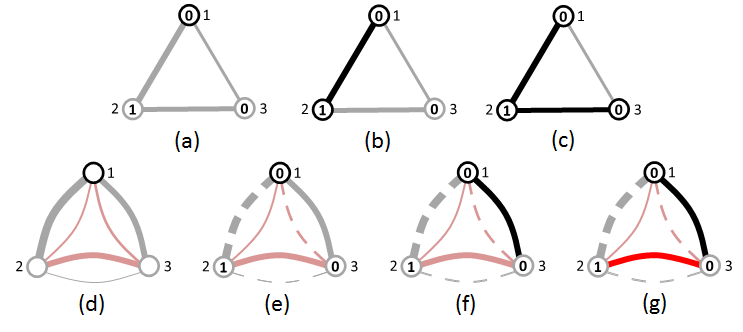
\includegraphics[width=3.4in]{AMWCS}
\caption{(a)  and (b) to (d) show the construction of  one-edge graph and two-edge graph, respectively. The value in each node represents the allele. The width of each edge corresponds to the strength of dependency measure between pairs. For (b) to (d), the gray and black edges represent the L(00$\cup$11) edge, while the pink and red edges represent the L(01$\cup$10) edge. Nodes and edges with color black or red represent the determined AMWCS.}
\end{figure}


Figure 1 depicts different results of model construction with  a problem of three bits, and a receiver with alleles $\{0, 1, 0\}$. First, the node 1 with allele 0 was randomly chosen from the candidate set $\{1, 2, 3\}$. For the one-edge scheme in Figure 1(a), node 2 is selected with the strongest edge $\{1, 2\}$. After two iterations, the inserted node sequence of the AMWCS  is $Q = \langle\{1, 2, 3\}\rangle$, and the ILS is  $\langle\{1\}, \{1, 2\}, \{1, 2, 3\}\rangle$. For the two-edge scheme in Figure~2(b), although there is a strong gray edge between nodes 1 and 2,  the pattern 10 conflicts with the meaning of the gray edges L(00$\cup$11). According to the linkage selection rule, the thin red edge $L(01\cup10)$ represents the linkage between nodes 1 and 2 with pattern 01. Therefore, after a receiver is determined in Figure 2(c), we remove all the conflict edges for clarity. Unlike the one-edge scheme, node 3, with the strongest edge $\{1, 3\}$, is picked in Figure 2(c). The inserted node sequence of the AMWCS is $Q = \langle\{1, 3, 2\}\rangle$,  and the ILS is $\langle\{1\}, \{1, 3\}, \{1, 3, 2\}\rangle$. In Figure 2(d), a receiver with pattern 001 and a random start node 1 are used in the two-edge graph construction. When another receiver is chosen, different conflict edges are removed, resulting in a customized ILS. Although the resulting ILS  $\langle\{1\}, \{1, 2\}, \{1, 2, 3\}\rangle$ is the same as one-edge graph in Figure 1(a), the two-edge graph is only constructed with non-conflict edges. 

Consider a longer instance with an optimal subsolution 111 similar to the three-bit problem in Figure 1. Strong linkages can be detected among these three bits. Following the procedures described above, the one-edge graph constructs the ILS as $\langle\{1\}, \{1, 2\}, \{1, 2, 3\}\rangle$. However, None of mask in the ILS can flip the receiver with pattern 001 to 111. In short, even if one-edge graphical linkage model detects the correct model, it might still fail during mixing since the pattern might not be the optimal subsolution. On the other hand, two-edge graphical linkage model  handles this problem by taking the alleles of receivers into account and preserve the correct pattern during mixing. For the two-edge scheme, choosing the mask $\{1, 3\}$ can help flipping the pattern 010 to the optimal subsolution 111.   

We believe that the ratio of a pattern in the population corresponds to the possibility of such pattern being the optimal subsolution. The two-edge model tends to align the alleles of receiver  with the dominant patterns in the population. The reason for such tendency lies in the characteristic of mutual information. Since the mutual information between two bits is divided into two parts in the two-edge graph,  the  linkage containing the high-ratio pattern  is always positive, while the other part is often negative.  In the example above, if the optimal subsolution 111 is prominent in the population, then the linkages $L(00\cup11)$ among these nodes should be positive, and the linkages $L(01\cup10)$ are likely negative.  



\begin{figure}
\centering
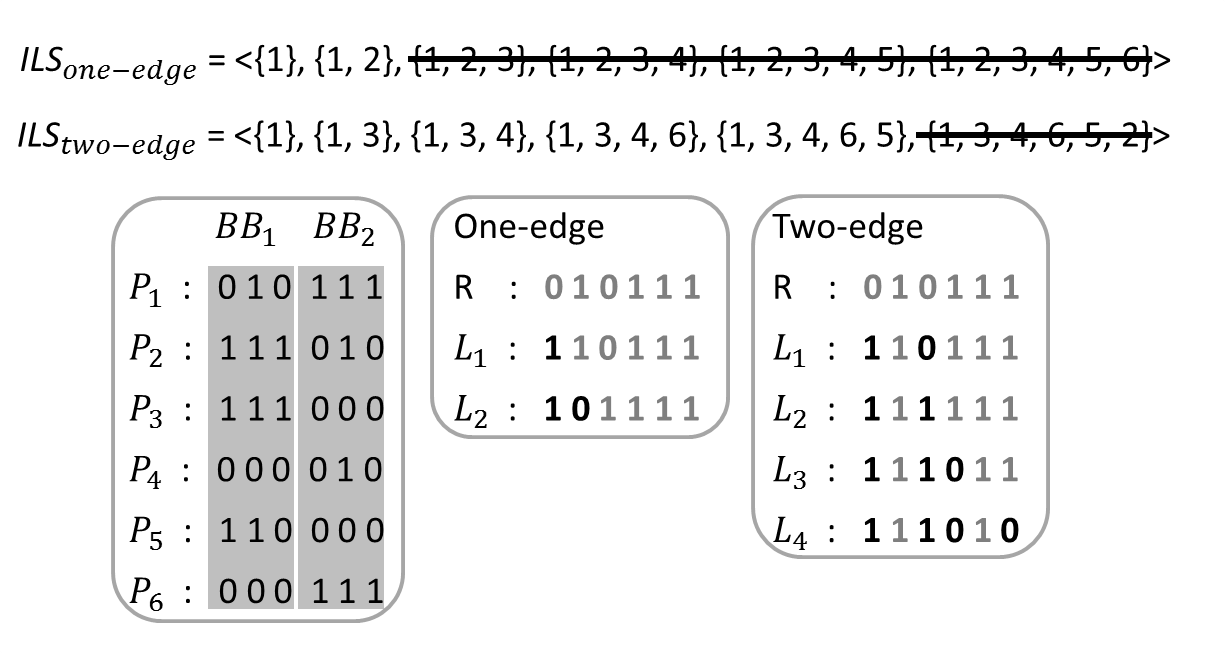
\includegraphics[width=3.4in]{SupplyBound}
\caption{Population $ P $ is on the left, and receiver $ R  = P_{1} $ is on the right. For both building-blocks 1 and 2, the subproblem optimal pattern is 010, and the suboptimal patterns are 000, 111. Masks with no supply of complement patterns are crossed out. Restricted mixing adopting the one-edge ILS stops at $ L_{2}$ due to lack of supply for longer masks. Restricted mixing adopting the two-edge ILS stops at $ L_{4} $ since a chromosome with equal fitness is generated.}
\end{figure}




\subsection{Supply bound}
Although taking the receivers into account enhances the effectiveness of bit-flipping, we notice the two-edge scheme costs more evaluations in the mixing stage, especially during the back mixing. The reason behind this phenomenon is \textit{supply overfitting}. After selecting an edge in the two-edge graph, the possible patterns for each pair of bits are narrowed down to either $\{00, 11\}$ or $\{01, 10\}$. Besides, we choose the node that gives the maximum linkage during model construction, meaning that the two selected patterns should have higher ratio in the population. Therefore, given a model constructed by a two-edge graph implies a higher possibility of finding the complement pattern in the population. The models that are customized for a specific receiver have a greater chance to pass the supply check. 


Figure 2 demonstrates the supply bound difference between one-edge graph and two-edge graph for a receiver 010111. The one-edge graph has shorter supply length since the complement patterns do not exist in the population. The two-edge graph is customized for the receiver, thus has a higher possibility in finding the complement patterns. Compared to the model constructed by one-edge graph, the masks in the two-edge ILS are more likely to pass the supply check. 


\begin{table}[t!]
\begin{tabular}{|c|c|c|c|c|}
\hline
 &
\multicolumn{2}{c|}{Supply length} &
\multicolumn{2}{c|}{Failure NFE in BM} \\
\hline
Problems  & One-edge & Two-edge & One-edge & Two-edge \\\hline
NK-S1 &  6.9 &12.6  &43.4 & 51.3 \\\hline
NK-S3 & 6.9  & 13.2  &42.3 & 48.8 \\\hline
NK-S5 & 2.6  &6.7  &  8.9& 10.1 \\\hline

\end{tabular}
\caption{Supply length and Back Mixing failure comparison (unit : K evaluations).}
\end{table}


The customized model benefits the restricted mixing, but when the receiver becomes a donor during the back mixing, such customization often overfits the donor. The experiment results in Table 1 show that the average supply length of the two-edge graph is about twice longer than the one-edge counterpart. As a result, the supply bound from the two-edge graph fails to serve its original purpose: limiting the recombination trials. In addition, the unnecessarily long patterns cause evaluation wastes and/or cross competition during the back mixing. 


To prevent the supply bound from overfitting the donor, we adopt the supply length of the one-edge graph as the supply bound. The major difference is that the linkage measure in the one-edge graph is calculated with complete mutual information, which gives the global information of the population. On the other hand, the linkage measure in the two-edge graph is more skewed that favors the given receiver during model building. Therefore, using the supply bound of the one-edge graph secures the global information between bits and does not overfit a specific chromosome. This gives a better result in back mixing and reduce NFE.


Furthermore, we also find the one-edge graph supply bound benefits the restricted mixing by enhancing the success rate of recombination. We speculate that in the early generations, subproblem patterns with better fitness do not stand out from the average patterns. The dependency information in the population is rather unclear. The inaccurate models then increase the probability of failure for the restricted mixing. However, the restricted mixing operator is only terminated when the supply bound is reached, or when the after-mixing fitness of the receiver is inferior to the original fitness. With the masks bounded by the one-edge graph supply length, unnecessary recombination trials can be reduced during the restricted mixing. 

%\begin{figure}[t!]
%\centering
%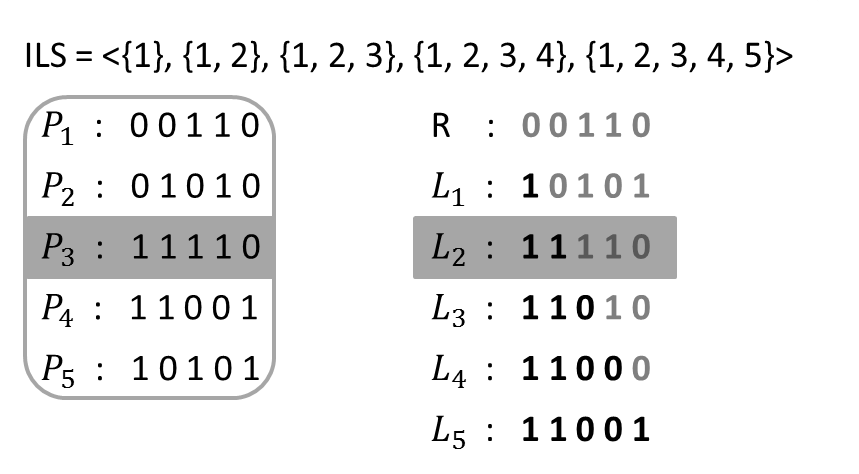
\includegraphics[width=3.1in]{IsinP}
%\caption{Early-stop criterion example.}
%\end{figure}


\begin{algorithm}[th!]
\caption{Modified Restricted Mixing}\label{algo_disjdecomp}

$ILS\_one$: one-edge incremental linkage set,\\
$ILS\_two$: two-edge incremental linkage set,\\
$f$: evaluation function, \\
$P$: population, $\ell$: problem size, \\
$T$: trial solution, $M$: mask, \\
${R_M}$: pattern of $R$ extracted by $M$, \\
${R_M}'$: complement pattern of ${R_M}$

\SetKwInOut{Input}{input}\SetKwInOut{Output}{output}
\Input{ $R$: receiver }
\Output{ $R$: reciever, $M$: mask }


\BlankLine
$ILS\_one  \leftarrow ConstructILS($one-edge$)$\\
$ILS\_two  \leftarrow ConstructILS($two-edge$)$
\BlankLine
\For{$i \leftarrow 1$ \KwTo $|ILS\_one|$} {
    $M \leftarrow ILS\_one_i$ \\
    \If {${R_M}' \not\subset P$} {
        $ SupplyBound \leftarrow i$
       
    }
}

\BlankLine
\For{$i \leftarrow 1$ \KwTo $|ILS\_two|$} {

    $M \leftarrow ILS\_two_i$ \\

    \If {${R_M}' \subset P$ and i < SupplyBound} {

        $T \leftarrow R$ \\
        $T_M \leftarrow {R_M}'$ \\

        \If {$T \in P$} {
            \Return ($R$, $\emptyset$) 
        }

        \If {$f(T) \geq f(R)$} {
            $R \leftarrow T$ \\
            \Return ($R$, $M$)
        }
    }
}
\Return ($R$, $\emptyset$) 
\end{algorithm}

%\subsection{Early-Stop Criterion}

%We propose a new early-stop criterion for the restricted mixing that eliminates unnecessary trials and reduces NFE. During the restricted mixing, the masks in the ILS are tried in an ascending order regarding to the mask size. If the new pattern gives worse fitness value than the original one, the receiver continues to try bit-flipping with the next  mask. This bit-flipping process stops only if the fitness of the generated chromosome is greater or equal to the fitness of the original receiver. However, this stop criterion might cost unnecessary evaluations since the recombination occasionally creates a chromosome that exists in the population. 



\begin{table*}[ht]
\centering
\newcommand{\tabincell}[2]{\begin{tabular}{@{}#1@{}}#2\end{tabular}}
\begin{tabular}{| c| c | c| c |}

\hline
Problems  & Equation & Problems & Equations\\\hline
 \tabincell{c}{Concatenated\\ trap} & 

\tabincell{c} {
$f_{m,k}^{trap}(x) = \sum_{i=1}^{m} f_{k}^{trap} \left (\sum_{j = i\cdot k-k+1}^{i\cdot k} x_j\right )$ \\
\\ 
$f_{k}^{trap}(u) =
   \begin{cases}
    1, & \text{if $u=k$} \\
    \frac{k-1-u}{k}, & \text{otherwise}\end{cases}$
}



&  \tabincell{c}{Folded \\trap}   &  \tabincell{c} {
\\
$f_{m,k=6}^{folded}(x) = \sum_{i=1}^{m} f_{k=6}^{folded} \left (\sum_{j = i\cdot k-k+1}^{i\cdot k} x_j\right )$\\
\\
  $f_{k=6}^{folded}(u) = 
   \begin{cases}
    1, 		& \text{if $|u=3| = 3$} \\
    0.8, 	& \text{if $|u=3| = 0$} \\
    0.4, 	& \text{if $|u=3| = 1$} \\
    0, 		& \text{if $|u=3| = 2$} \\
	\end{cases}$
\\
\\
}
\\\hline
 
\tabincell{c}{Cyclic\\ trap} & \tabincell{c}  {
\\
$f_{m,k}^{cyclic}(x) = \sum_{i=1}^{m} f_{k}^{trap} \left (\sum_{j = i\cdot(k-1)-k+2}^{i\cdot(k-1)+1} x_j\right )$\\
\\
 $f_{k}^{trap}(u) = 
   \begin{cases}
    1, & \text{if $u=k$} \\
    \frac{k-1-u}{k}, & \text{otherwise}
	\end{cases}$
\\
\\
}

&NK-landscape   &  \tabincell{c}{  
$f_{\ell,k,s}^{NK}(x) = \sum_{i=0}^{(\ell-k-1)/s}$\\
\\
$ f_{k,i}^{subNK} (x_{i{\cdot}s+1},x_{i{\cdot}s+2},...x_{i{\cdot}s+k+1})$}
\\\hline
2D Spin-glass & $f_{n}^{spin}(x) = -\sum_{i,j=0}^{n} x_{i}x_{j}J_{ij}$  &MAX-SAT   &   $F = \bigwedge_{i=1}^{m} \left (\bigvee_{j=1}^{k_{i}} \ell_{ij} \right )$\\\hline

\end{tabular}
\caption{Equations of the benchmark problems}
\end{table*}

%For example, consider a five-bit trap problem with global optimum 11111 and local optimum 00000 in Figure 3. $P_{1}$ is chosen as receiver in the restricted mixing. Suppose the masks in ILS follow the sequence $\{1, 2, 3, 4, 5\}$ and the complement patterns for all five models exist in the population. Restricted mixing failed with mask $\{1\}, \{1, 2\}$ since the patterns are inferior to the original pattern 00110 in trap problems. After performing bit-flipping with the second mask $\{1, 2\}$, the resulted pattern 11110 exists in the chromosome $P_{3}$. The original stop criterion continues the procedure, ending up with three more failure recombinations, $L_3, L_4,$ and $L_5$. 
%These attempts are unnecessary, since now they can be performed on the existing chromosome $P_{3}$. 
%Also, such unnecessary attempts may cause other chromosomes similar to $P_3$ and undesirably reduce the diversity of the population.


%To prevent from this situation, we terminate the restricted mixing whenever the new generated chromosome already exists in the population. Another receiver along with another set of customized models are chosen for the next iteration of the restricted mixing. This criterion preserves diversity in the population and also reduces NFE waste. The pseudocode of the modified restricted mixing is given in Algorithm 4.

\section{EXPERIMENT RESULTS}
In this section, we first briefly introduce the six benchmark problems for the following experiments. Then, the experiment setup is detailed. Finally, we compare and contrast the experiment results of the original DSMGA-II, the modified DSMGA-II, LT-GOMEA and hBOA. 


\subsection{Test Problems}
Six types of linkage benchmark problems are used in this paper, including four classical linkage-underlying problems and two real-world problems. These benchmark problems each covers different aspects and characteristics of real-world problems. The \textit{Concatenated Trap} is composed of $m$ additively separable trap functions, each with $k$ variables~\cite{deb:sufficient}. It is well known that in order to solve trap problems, the underlying structure must be detected and preserved during mixing~\cite{thierens:mixing}. The \textit{Cyclic Trap} consists of overlapping trap functions with wraparound~\cite{yu:overlapping}. The \textit{Folded trap} is one of the multiple variants of \textit{NK-landscape} problems described in~\cite{goldberg:deception}. We use the bipolar deceptive function with the subsolution size $k = 6$. 
%Each subsolution contains two global optima and lots of local optima. 
The performance depends heavily on the ability of reducing unnecessary exploration of plateaus due to the symmetric characteristics of the trap function. 
The \textit{NK-landscape} functions are composed of overlapped and randomly generated sub-functions~\cite{pelikan:overlap}. 
Each instance is controlled by three parameters: the problem size $\ell$, the number of neighbors of one gene $k$, and the step size $s$, i.e. the offset of two adjacent sub-functions.
We use \textit{NK-landscape} with step 1, 3 and 5 to represent problems with different degrees of overlapping in our experiments.

The \textit{Ising spin-glass} gives a set of variables in one of the two states \{+1, -1\}.
For each pair of neighboring spins $i$ and $j$, there exists a coupling constant $J_{ij}$.
The goal is to find a combination of states that satisfies the most coupling pairs.
We also use the classical NP-complete \textit{Maximum Satisfiability problem} (MAX-SAT).
For our experiments, we use the Uniform Random-3-SAT instances from SATLIB\footnote{http://www.satlib.org} with all satisfiable clauses.



\subsection{Experiment Setup}
DSMGA-II is an enhanced edition of DSMGA and it outperforms multiple variants of its predecessor~\cite{yu:DSMGA} in all benchmark problems. 
Thus, we will not discuss DSMGA in the following comparison.
DSMGA-II is based on the idea of OM, so it is necessary to compare DSMGA-II with GOMEAs. 
In our experiments, we use the version of LT-GOMEA with forced improvement \footnote{http://homepages.cwi.nl/$\sim$bosman/source\_code.php}.
Although several different linkage models have been proposed over the years~\cite{bosman:robust}, LT-GOMEA~\cite{bosman:LT-GOMEA} is still considered a state-of-the-art OM algorithm.
Also, we compare DSMGA-II with the hierarchical Bayesian optimization algorithm (hBOA)~\cite{pelikan:hBOA}
Similar to LT-GOMEA, hBOA is also a milestone and is often used in recent Model-Building GA researches.


A minimum population is required for a certain number of consecutive successful runs.
However, the conventional bisection procedure~\cite{pelikan:hBOA} often fails to yield the minimum NFE  since the minimum population size varies in the bisection procedure for different algorithms.
In the following experiments, we adopt an adaptive sweeping procedure described in~\cite{hsu:DSMGA2} for more accurate search of minimum NFE.
%The sweeping procedure starts with a reasonable population size.
%If the algorithm cannot consecutively reach the global optimum with the given population, the population size increases with a predefined step.
%In this paper, The initial population size is set to 10, and the initial step is 30.
%A successful trial is defined as 10 consecutive successful hits.
%The mean of NFE over 10 successful runs is recorded as the minimum evaluations required for a given population size.
%After a successful trial is recorded, a smaller step is adopted to narrow down the sweeping range.
%The sweeping procedure continues until the step converges.
%In this paper, we divide the step by 2 for each iteration, and the procedure terminates if the sweeping range is within 5\% of the population size.
The sweeping procedure gives better precision than the canonical bisection procedure, since the acquired resolution increases as the steps decreases after each successful trial.
The minimum evaluations required for each problem are averaged over 100 independent runs or instances.

We compare DSMGA-II, LT-GOMEA, and hBOA under the following settings. 
The selection pressure is set as 2 for all three algorithms. 
For DSMGA-II, the constant $R$ in Algorithm 1 is set to be $\ell/50$, as suggested in~\cite{hsu:DSMGA2}.
LT-GOMEA is performed without local search to enhance its performance, as in~\cite{bosman:LT-GOMEA}.




\subsection{Results and Discussions}

Now we compare the modified DSMGA-II with the original one. The following comparisons are divided into three categories based on different characteristics of the problems. Our comparison focuses on the modifications differed from the original DSMGA-II. For reference, however, we also include the results of hBOA and LT-GOMEA. 

\subsubsection{ Comparison on deceptive variants }


We first consider the deceptive problems. The results are shown in Figure~\ref{fig:trap}.
For the concatenated trap problem, there is little difference between the modified DSMGA-II and the original. It is because that the problem structure is relatively easy for DSMGA-II to learn, both subsolutions, 00000 and 11111, are clearly identified in the early stage. As a result, the edge $L(01\cup10)$ is rarely used. 


For the cyclic trap problem, the two-edge graph helps the linkage model grow toward to the correct direction. For instance, consider the pattern ``1111\textbf{0}0000'', and the ILS construction starts from the middle 0. The two-edge graph suggests the linkage mask to connect its right neighbor instead of its left neighbor since $L(01\cup10)$ is much weaker than $L(00\cup11)$ for the trap function. Therefore, a moderate evaluation reduction is achieved. 

For the folded trap problem, the two-edge model helps aligned the receiver with the prominent pattern in population. The modified version more likely flips the plateau (such as 111000) to the correct subsolutions (000000 or 111111) than DSMGA-II with the original DSM. As a result, significant improvement can be produced. 



\begin{figure}
\centering
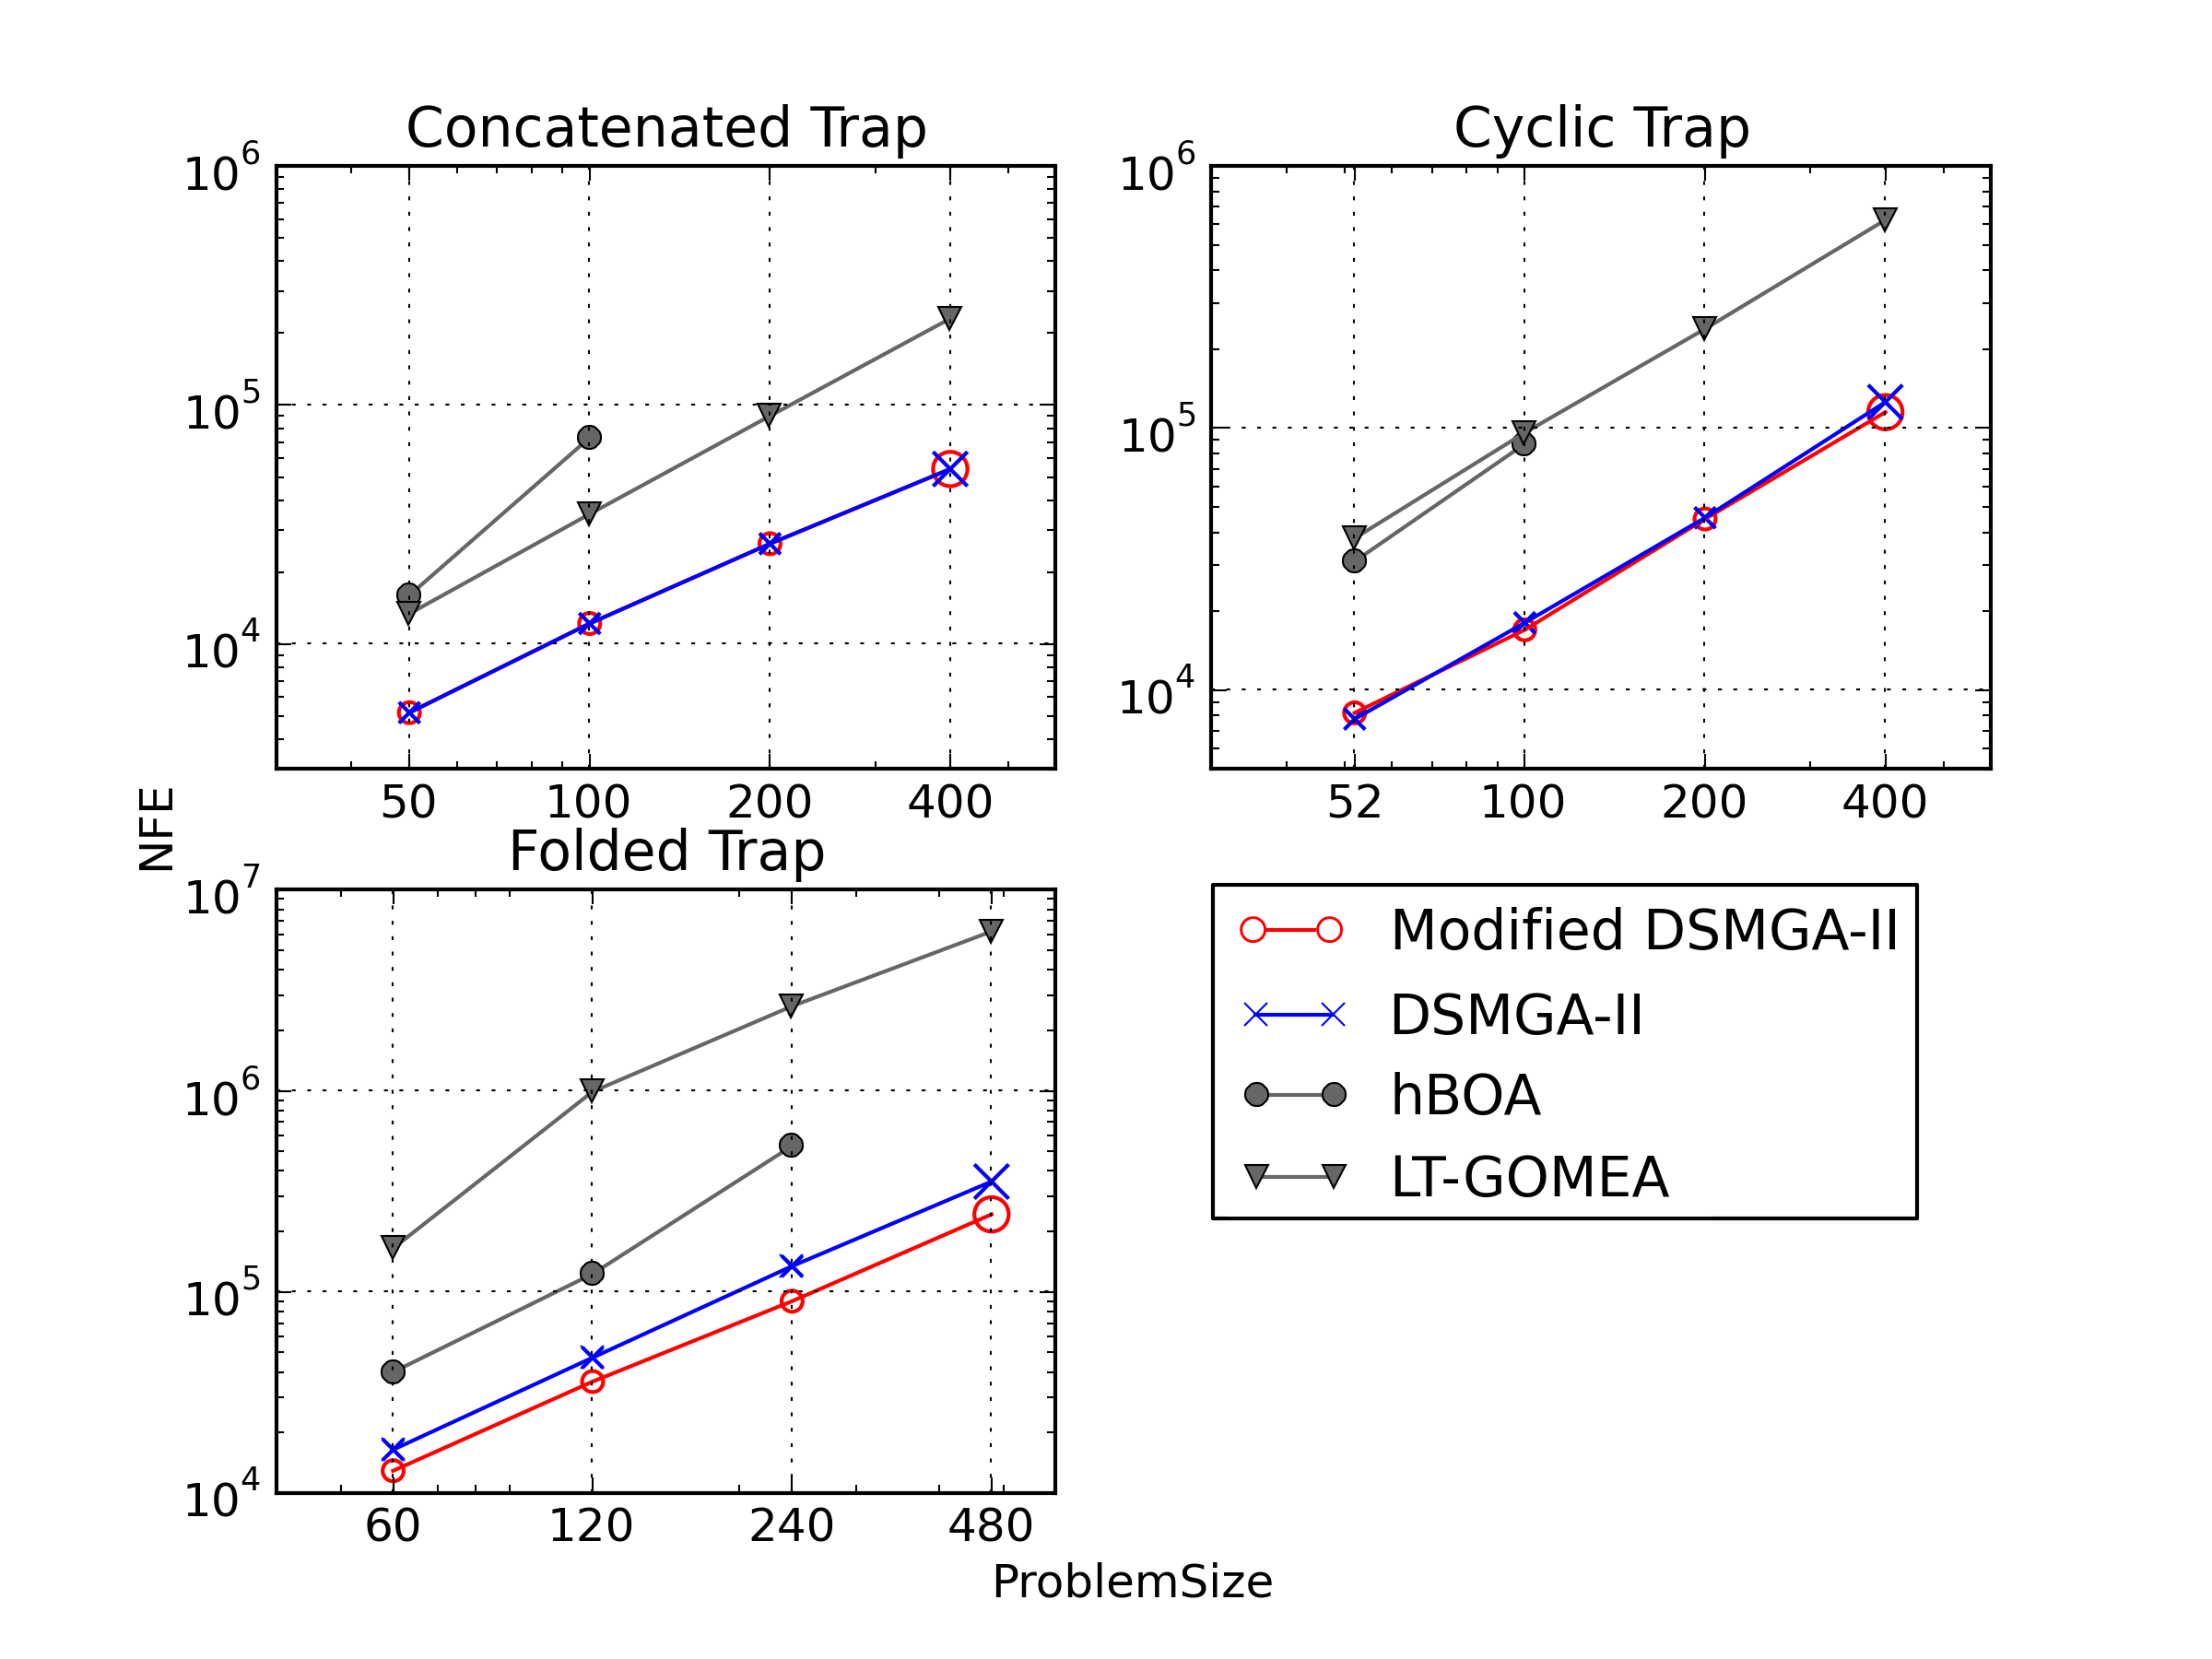
\includegraphics[width=3.3in]{trapResults}
\caption{Scalability of the modified, the original DSMGA-II, LT-GOMEA and hBOA on the problems of deceptive variants.}
\label{fig:trap}
\end{figure}


\subsubsection{Comparison on the NK-landscape problems}

\begin{figure}
\centering
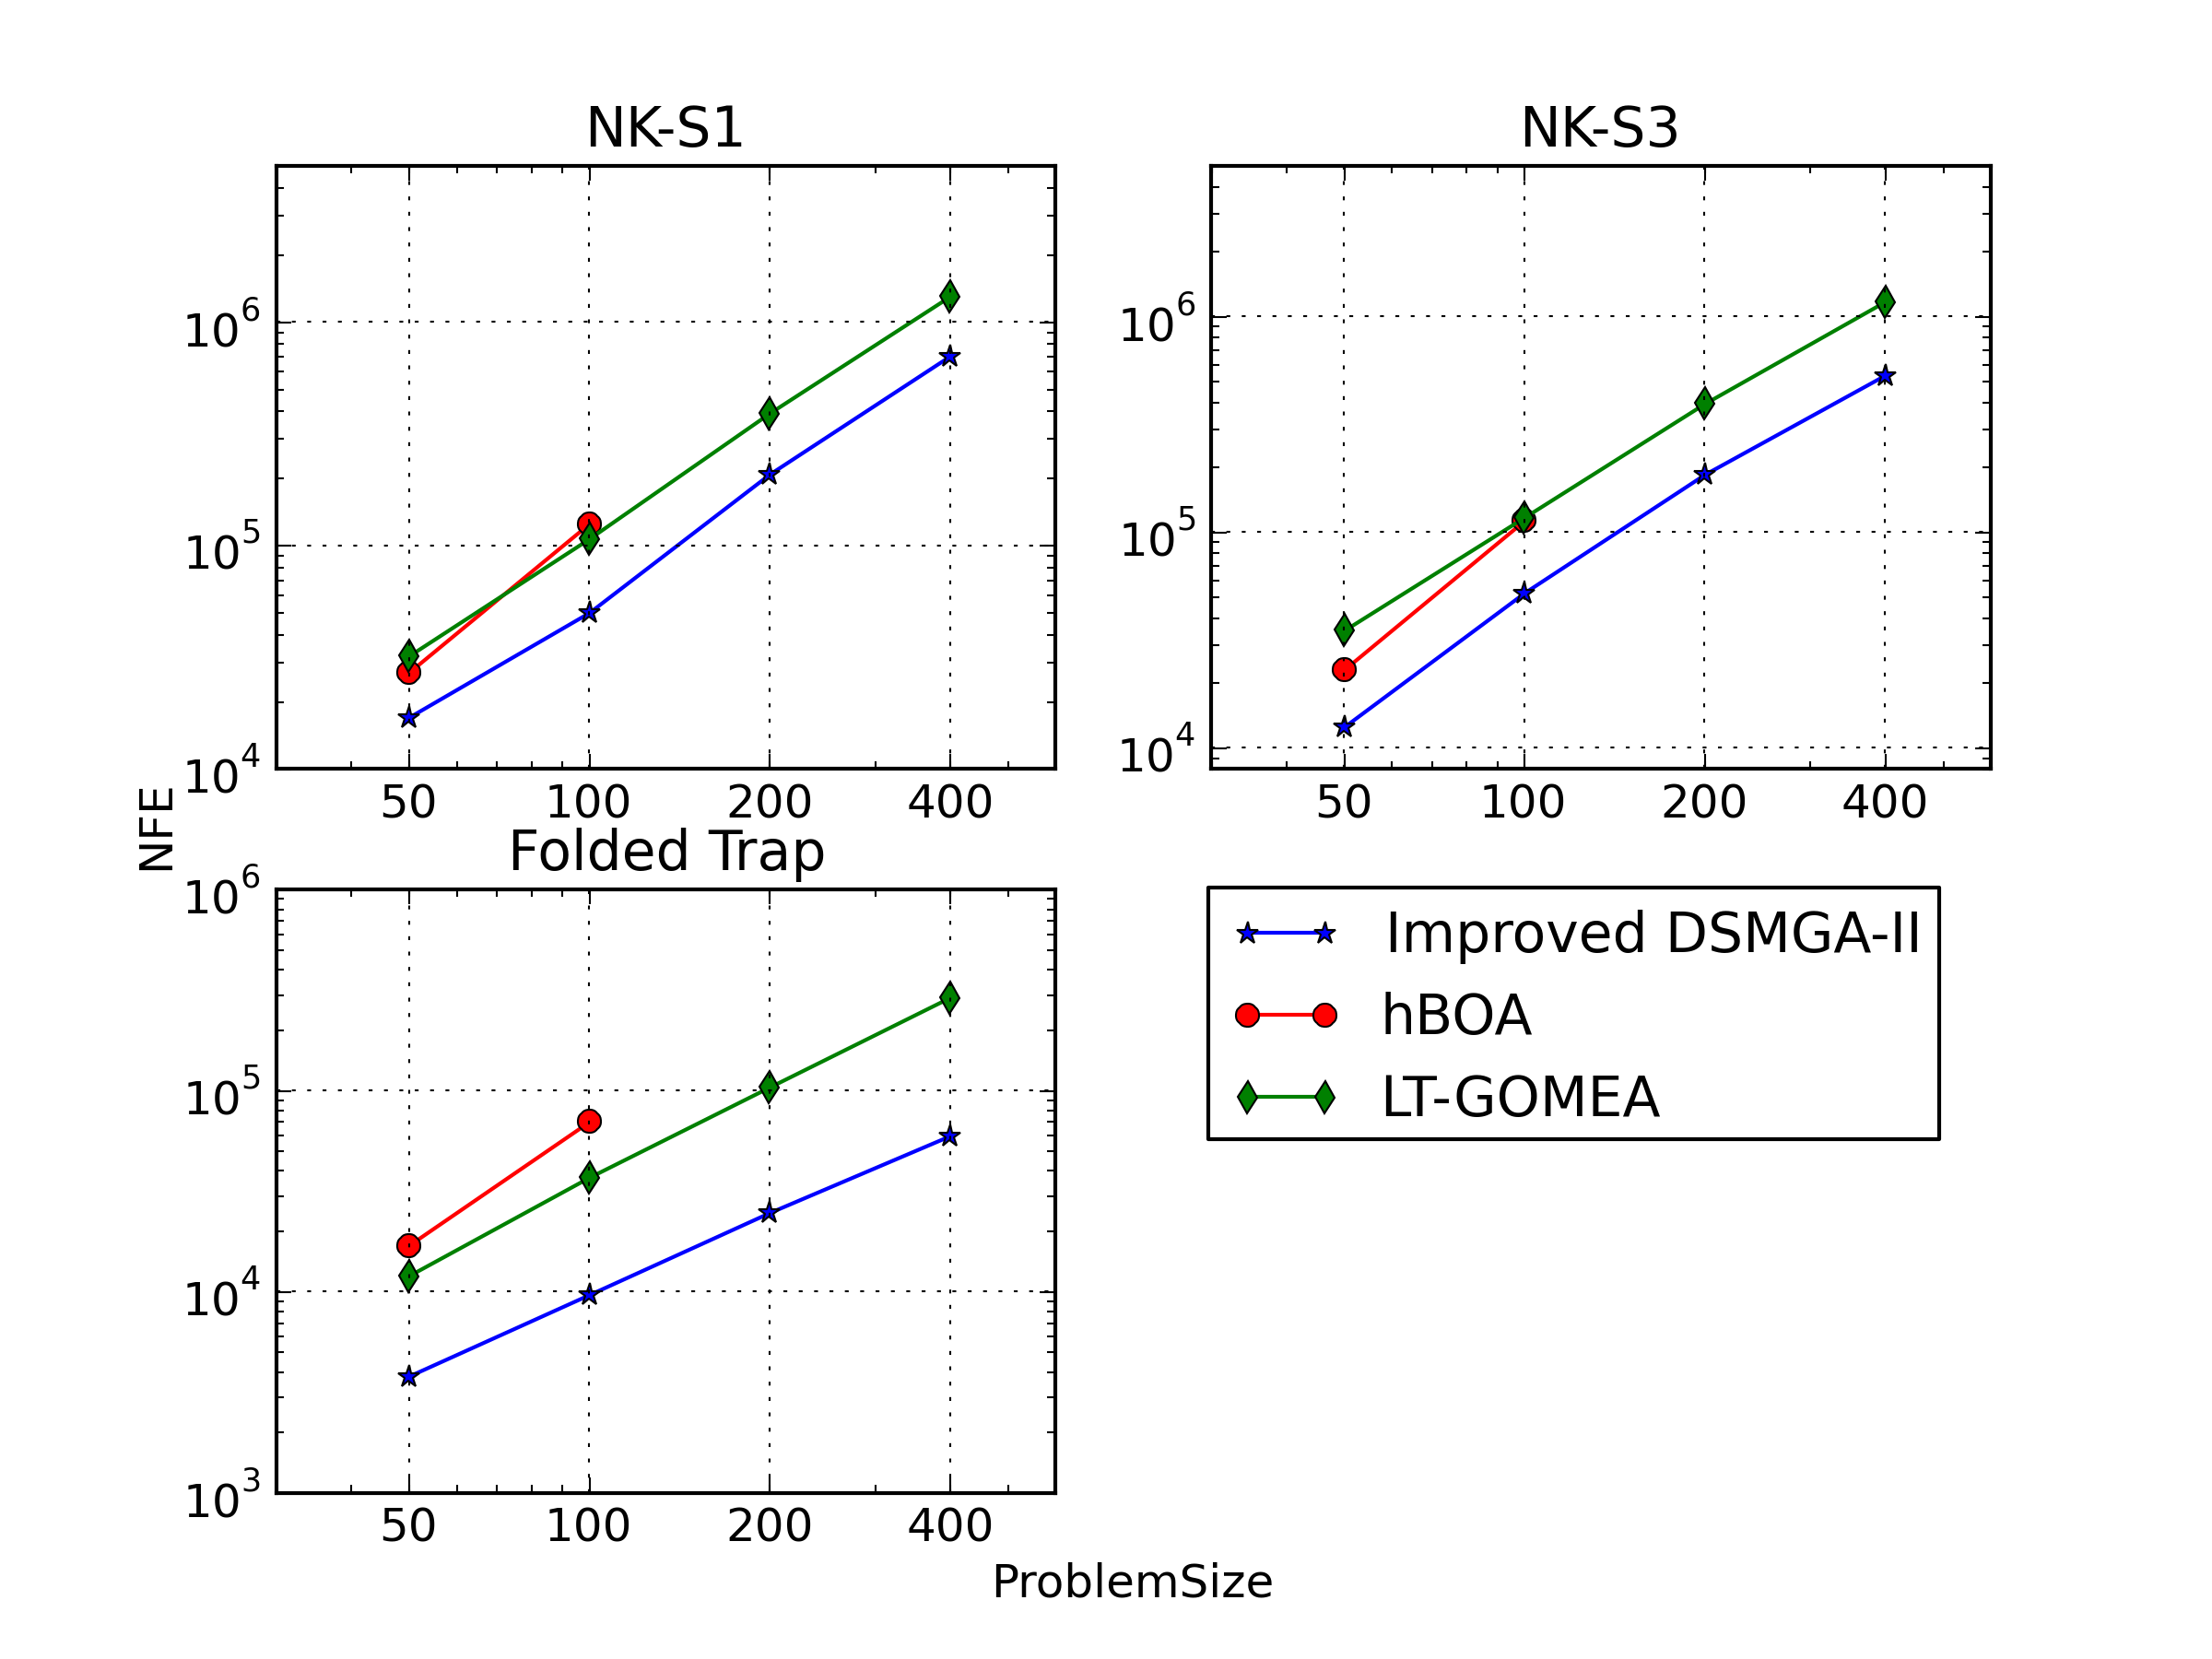
\includegraphics[width=3.3in]{nkResults}
\caption{Scalability of the modified, the original DSMGA-II, LT-GOMEA and hBOA on NK-landscape with various degrees of overlapping.}
\end{figure}


The results of the NK series (Figure~5) demonstrate the ability of the ILS model in handling randomly generated overlapping problems. 
The difference between the modified DSMGA-II and other algorithms enlarges as the degree of overlapping decreases. 
Our modifications do not improve DSMGA-II by much since the NK problems do not have clear structures to for two-edge graph to exploit. Nevertheless, our modifications still maintain the performance of the original algorithm. 

\subsubsection{ Comparison on two real-world problems }

For the Ising spin-glass problem (Figure~6), the slope of DSMGA-II decreases as the problem size increases. 
This is due to the numerous numbers of plateaus in the spin-glass problem.
As for the MAX-SAT problem, while the NFE grows exponentially, which is reasonable since MAX-SAT is known to be NP-hard, the modified DSMGA-II still requires the fewest evaluations among all the algorithms. To sum up, the modified version yields fewer evaluations and better scalability on both problems. 

\begin{figure}
\centering
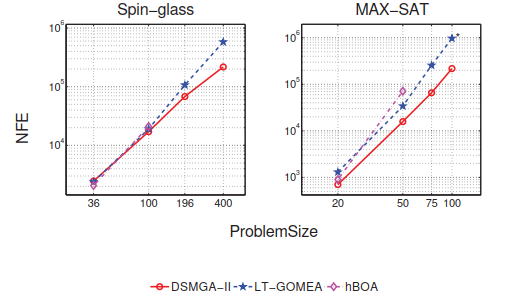
\includegraphics[width=3in]{spin_satResults}
\caption{Scalability of the modified, the original DSMGA-II, LT-GOMEA and hBOA on Spin-glass and MAX-SAT.}
\end{figure}

\subsubsection{ Comparison with the original DSMGA-II }

\begin{table*}[ht]
\centering
\label{my-label}
\begin{tabular}{lclcclcclllr}
\hline
              &        &  & \multicolumn{2}{c}{Original} &  & \multicolumn{2}{c}{Modified} &  &       		&					&         		\\ \cline{4-5} \cline{7-8}
Problem       & $\ell$ &  & M            & SD            &  & M            & SD            &  & t			& Sig.(2-tailed)	& Improvement  \\ \hline
Concat. trap  & 400    &  & 55.0         & 7.9           &  & 53.6         & 6.9           &  & 0.25   		& .804				& 2.52\%  \\
Cyclic trap   & 400    &  & 123.2        & 18.8          &  & 113.2        & 13.7          &  & 2.75	  	& .007				& 8.13\%  \\
Folded trap   & 480    &  & 354.6        & 11.4          &  & 243.7        & 6.0           &  & 105.18 		& .000				& 31.27\% \\
NKs1          & 400    &  & 767.4        & 418.0         &  & 713.7        & 376.5         &  & 1.66     	& .100				& 7.00\%  \\
NKs3          & 400    &  & 550.6        & 210.8         &  & 533.5        & 230.0         &  & 0.17  	   	& .869				& 3.10\%  \\
NKs5          & 400    &  & 62.1         & 6.3           &  & 59.5         & 5.1           &  & 2.73  		& .007				& 4.08\%  \\
MAX-SAT       & 200    &  & 7887.6       & 12470.6       &  & 6291.3       & 10689.5       &  & 3.39    	& .001				& 20.24\% \\
2D spin-glass & 784    &  & 863.2        & 505.0         &  & 683.3        & 321.4         &  & 3.99		& .000				& 20.85\% \\ 
\hline 
%***$p<.005$. \\
\multicolumn{12}{l}{$Note.$ $\ell$ = Problem Size. M = Mean. SD = Standard Deviation. t = paired t-test statistic.} \\
\multicolumn{12}{l}{Improvement = $1 - \mu_{Modified}/\mu_{Original}$. }
\end{tabular}
\caption{Required NFE of DSMGA-II for the largest test problems (unit : K evaluations)}
\end{table*}



Some of the improvements may not easily be observed from the above figures due to the logarithmic scale. Here we list the NFEs required to solve the largest problems in Table~3.  Compared with the original DSMGA-II, the modified version shows superior performance on all benchmark problems except the concatenated trap problem. The NFE reduction reaches up to 30\% when dealing with the folded trap problem.

The two-edge graph constructs customized models for a chosen receiver. 
This characteristic shows advantage when facing problems with plateaus.
Since the two-edge model tends to align with the most prominent pattern in the population, fewer evaluations are needed to jump out of plateaus due to stronger drifting effect. This characteristic also helps when solving the Ising spin-glass problem. 
There are often two equal-fitness subsolutions in the spin-glass problem.
The original DSMGA-II can only detect the strong linkage of the subsolution without knowing the correct pattern of the subsolution to contribute to global fitness.
This results in a significant waste of function evaluations on repeatedly flipping subsolution patterns to another equally fit subsolution.
With the two-edge graph, different models can be generated from the same graph. 
Empirically, this helps preserve the optimal patterns during mixing and reduce attempts of trying the complementary pattern.



\section{Conclusions}
 
In this paper, we proposed a two-edge graphical linkage model for DSMGA-II. 
The new model is more expressive than the original one and provides customized recombination masks for every single chromosome. 
To reduce unnecessary function evaluations, a new criterion of supply check  is also designed. Combined with the other minor modification, the early stop, the new linkage model shows a stable scalability and improves the original DSMGA-II by up to 30\% in terms of NFE.



Researches concerning model-building techniques, providing centralized information for recombination, have improved the canonical genetic algorithms by much. 
We find it interesting that distribution of such centralized techniques (customization the recombination for each chromosome) again can improve the performance of model-building genetic algorithms. 
Such improvement may be applied to other evolutionary algorithms as well; of course,  further investigations, especially from the theoretical aspect, are needed.  


\begin{acks}
The authors would like to thank the support by Ministry of Science and Technology in Taiwan under Grant
No.~\grantnum{}{MOST 105-2221-E-002-191}.
\end{acks}
